%Appendix -- January 2015 appendix

\renewcommand{\chaptername}{Appendix}
\renewcommand{\thechapter}{A}


\chapter{The good, the bad and the ugly of RbLi}
\label{app:RbLi}

This appendix summarizes the best, the worst and the meh aspects of the RbLi apparatus. Hopefully the items presented here are helpful to future students building experimental apparatuses for ultracold atoms.  

\section{The good}

It is very easy to come up with a list of bad things that don't work quite well in the lab. Coming up with a list of good things that work well is harder; if we are not fixing a broken thing we don't think much about it. When the current postdoc was prompted with the question of what she loved most about our apparatus she answered `I love every single thing about RbLi.' Unfortunately there is not enough space to talk about every single thing and the list below summarizes some good things in our lab.

{\bf Overkill transistor banks:} Large currents in the lab (quadrupole and Zeeman slower) are controlled with MOSFET banks formed by a group of MOSFETS whose drain and source are connected in parallel and sharing the same gate voltage that is controlled by a PI servo. The Zeeman slower always operates at a fixed current but the current in the quadrupole coils is dynamically changed throughout the experimental sequence and a fast response is desirable.
In 2013 we replaced the quadrupole MOSFET bank with a new unit that contains 20 \noted{IXFN 520N075T2} transistors rated for $\unit[75]{V}$and $\unit[480]{A}$ (left panel of Figure~\ref{fig:transistor_specs}). Even though our currents never exceed $\unit[70]{A}$, the performance of the transistors really decays as the drain to source voltage is increased as can be seen in the right panel of Figure~\ref{fig:transistor_specs}. The use of more transistors reduces the power dissipation of each individual transistor which allows us to operate the power supply at a higher voltage of $\unit[15]{V}$ that helps counteract the inductive kickback of the coils. With the new transistor bank the turn on time of the coils was reduced from $\unit[100]{ms}$ to $\unit[50]{ms}$ leading to improved magnetic trapping and better Stern-Gerlach pulses for imaging, only with an unavoidable small number of blown off transistors. 

\begin{figure*}[htb]
\begin{center}
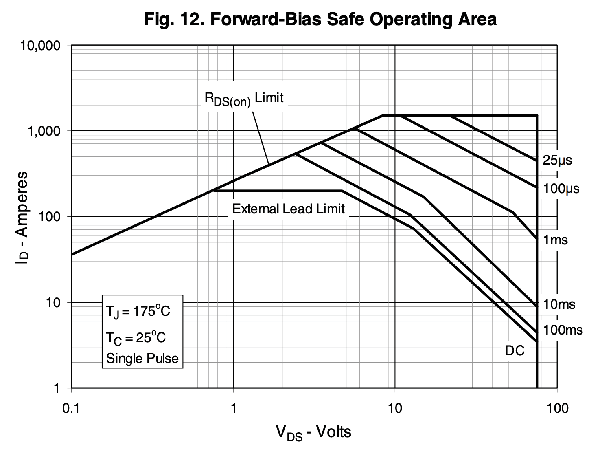
\includegraphics[]{Figures/AppendixA/transistor_specs.pdf}
\caption[New MOSFET bank]{Left: New MOSFET bank. Right: Safe operation regime of the \noted{IXFN 520N075T2} MOSFET. Even though they are in principle rated for up to $\unit[480]{A}$ the maximum safe current is greatly reduced at larger drain to source voltages $V_{DS}$. A high $V_{DS}$ is desirable to reduce the inductive kickback during turn on.}
\label{fig:transistor_specs}
\end{center}
\end{figure*}

{\bf Hand made in vacuum shutters:} Before going into the Zeeman slower, the atoms that were heated in the Rb oven travel to the main oven chamber that is pictured in Figure~\ref{fig:RbLi}b containing a cold-cup and an oven shutter. The cold-cup is a cylindrical shaped copper piece that is attached to the cold end of a thermo-electric cooler (TEC) via a copper rod. We keep the cold-cup temperature at $-\unit[30]{C}$ in order to capture excess Rb atoms in the chamber and prevent damaging the ion pumps. The oven shutter allows us to block after the MOT loading stage to prevent unwanted heating. We use a homemade device, made from a re-purposed hard drive disk shutter with a metallic flag attached to its end. The shutter is electrically connected to en electric feedthrough with vacuum-compatible Kapton sealed wires. Other apparatus within the JQI~\cite{BrownThesis} have commercial shutters from \noted{Uniblitz} and some of them have failed in the past. Overall we have found this setup to be very reliable. The only problem we experienced once was some accumulation of Rb on the cold cup that started blocking the atomic beam. To remedy this we reversed the polarity of the TEC and heated the cold cup barely enough so that the accumulated Rb atoms melted and moved away from the aperture of the atomic beam. 

\begin{figure*}[htb]
\begin{center}
\includegraphics[]{Figures/AppendixA/oven_chamber.pdf}
\caption[The RbLi oven chamber]{The RbLi oven chamber. We use a homemade in-vacuum shutter to block the atomic beam after the MOT stage to prevent heating of the atoms at later stages.}
\label{fig:RbLi}
\end{center}
\end{figure*}

{\bf Ultraviolet LEDs:} We have two $\unit[3]{W}$ ultraviolet LEDs from \noted{Mightex} placed at the glass cell side of the vacuum system. One is aimed at the vacuum window where the slower beam enters and the other is placed aiming at the glass cell. The LEDs prevent Rubidium from depositing on the vacuum system and can conveniently be turned on and off with a TTL signal from the computer. We have found that routinely turning them on (for example, leaving them on overnight) leads to a smoother operation of the system. 

{\bf Mirror mounts with picomotor actuators:} We use \noted{8816-6} picomotor optical mounts from \noted{New Focus Optics} whose deflection angle can be electronically adjusted on the order of microradians. The addition of picomotor mounts has made alignment of laser beams to the atoms significantly easier. We use this mounts on the last tunable mirror before the atoms for beam paths whose alignment is critical, for example in optical dipole trap and Raman beams. 

{\bf Polarizers on MOT beams:} The light of our MOT beams is coupled to polarization maintaining optical fibers. We found that besides our best efforts to align the polarization of the incoming light to the axis of the fiber the fluctuations in the output polarization could cause considerable instabilities in the BEC production. To keep the polarization clean we placed polarizers at the output of the fibers. We found that despite the power hit we can get from the changes in polarization, this solution leads to a much more stable production of BECs. 

{\bf Lab couch:} When the experiment is functional enough that data can be taken long hours in the lab are often required. If it gets late, the lab couch allows the person running the experiment to take small naps as the data keeps coming while still being close to the apparatus in case something needs to be fixed. 

{\bf Other elements already mentioned in the main text:} The new master laser from Vescent photonics has been very stable and reliable. The new Mako camera has been very helpful to get rid of unwanted fringes in absorption images. Labscript makes writing experimental sequences very straightforward. 

% mica capacitors for high power RF impedance matching?

\section{The bad}

The bad, these are elements of the apparatus that were constant sources of pain and if considering a new experimental design should be avoided. 

{\bf Water cooling shared between two labs:} The quadrupole and Zeeman slower coils as well as the transistor banks require water cooling due to Joule heating. Our lab space is shared with a Rubidium-Ytterbium ultracold mixtures apparatus~\cite{HeroldThesis} and amongst the things we shared is the water cooling system. The schematic in Figure~\ref{fig:water_cooling} illustrates the layout of the water cooling system. The water was filtered at two different points, first at each line has a $\unit[440]{\mu m}$ particulate filter from \noted{Swagelok} and then the water returning to the heat exchanger is filtered with a low-impedance cellulose cartridge (\noted{McMaster 7191K11}). Both filters only capture impurities in the water for one given flow direction. One of the failure modes which occurs when one of the booster pumps is turned on before the heat exchanger, causing water to flow from one experiment to the other and bringing a collection of nasty things that escapes the filters into the coils. Over the years our system has suffered of clogged filters, clogged coils and broken booster pumps. For best operation it is highly recommended that the cartridge filter is changed and that the Swagelok filters be cleanded at least once a year and that a $10\%$ solution of an anti-corrosive \noted{Optishield Plus} in water is used as a coolant. Even when following this practices, we managed to find lots of gunk and unidentified objects (sand? glass? mud? oxide? dead bacteria?) in the water, just at a slower rate.

\begin{figure*}[htb]
\begin{center}
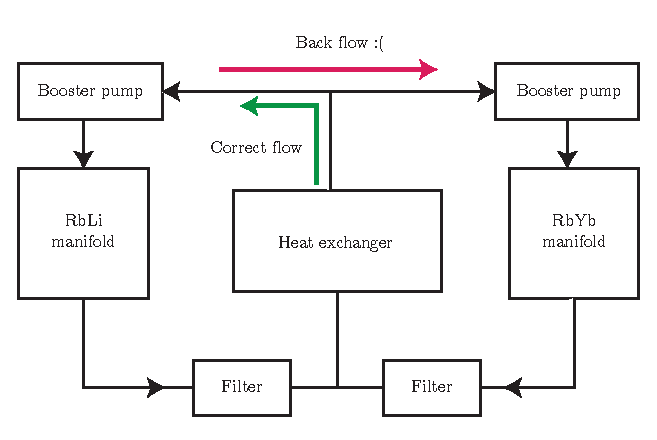
\includegraphics[]{Figures/Chapter4/water_cooling.pdf}
\caption[Water cooling manifold schematic]{Simplified schematic of the shared water cooling manifold.}
\label{fig:water_cooling}
\end{center}
\end{figure*}

{\bf Flipper mirrors:} The optical path of the MOT beams near the atoms is very close to that of Raman, optical dipole trap and probe beams. Since the MOT beams are only used at the early stages of the experiment it is tempting to use flipper mirror mounts so that once they are no longer needed they can be moved away to make space for other beams. This was the approach originally taken in the lab and we used \noted{8893-K} motorized optical flipper mounts from \noted{Newport} in multiple locations. As they break over and over again, they have been slowly replaced by more stable solutions such as periscopes or polarizing beam splitters wherever it is possible. Flipper mirrors are always bound to break, it is only a matter of time. Avoid using them unless you absolutely have no alternative. 

{\bf Optical fibers right below air vents:} The optical fibers connecting the main experiment optical table and the laser optical table are routed close to a pair of AC vents in the lab. The changes in air temperature result in polarization fluctuations at the output of optical fibers, a constant cause of pain and instability in our BEC production. We have tried to remedy this issue by partially blocking vents and enclosing the fibers in a large PVC tube. 

{\bf Free space dipole laser:} The laser system providing $\unit[1064]{nm}$ light for the optical dipole trap is not fiber coupled and is setup in the same optical table as the vacuum system; we are not able to change the laser without destroying the alignment of the beam with the atoms.  This issue became important while setting up a 1D optical lattice by retro-reflecting one of the dipole trap beams we noticed that the laser mode is not very stable, leading to big fluctuations in the optical lattice. In the original design of the laser system high-power photonic crystal fibers were included but they did not have built in mode expanders which resulted in the tip of the fiber inevitably getting burnt after some time of use. In short, mode expanders are recommended in applications involving large optical powers.

\section{The ugly}
The ugly elements are not quite bad but they don't function flawlessly either. If given the option to replace them with something better I definitely would. 

{\bf Kepco bipolar power supplies:} We use three \noted{Kepco BOP 20-20M} bipolar power supplies to provide the current for the bias coils. While it is nice to have a commercially available power supply that can provide $\unit[\pm 20]{A}$ they come with a few drawbacks. First the current they provide has $\unit[60]{Hz}$ noise in it and in order to suppress it and stabilize the currents we must use a PI feedback circuit. The power supplies has multiple banks of NPN and PNP transistors inside mounted on a big heat sink with fans attached to it making them quite noisy; it is not optimal to place them close to the main experiment chamber and long connections open the door to unwanted ground loops. Additionally they have a few failure modes. The most common problem we experienced was output current would rail, which is related to broken transistors which tend to inevitably fail after some time. Many of the symptoms of broken Kepcos spoken by other labs seem to usually boil down to malfunctioning transistors.  

{\bf Toptica's BoosTA:} Our cooling light comes from a \noted{Toptica DL Pro} is amplified using a \noted{Toptica BoosTA} tapered amplifier system. While the output power of this TA has been relatively stable over the years it has a tendency to turn itself off. On its bad days it would turn off so often that it would be impossible to operate the experiment. We haven't been able to identify the problem despite our best efforts to look into the TA controller, the TA itself, multiple conversations with Toptica engineers etc. 

{\bf Too many devices connected to the same computer:} We use multiple \noted{USB-6229} data acquisition (DAQ) devices from \noted{National Instruments}. They are located at different points of the lab and then connected to the control computer through USB to optical fiber adapters that break the ground between the computer and the rest of the lab equipment (a practice we always try to follow when connecting things to the computer). We have a total of 6 NI devices in addition to other equipment like oscilloscopes all connected to the computer through BNC cables. Often times we struggled with the computer failing to detect one or multiple devices and it would take a very special (and different every time) combination of plugging and unplugging, turning off and turning back on things until all devices were recognized by the computer. We observe that the problem occurs less often when we don't have as many USB devices connected to the computer. 



 